\section{GWFSS Competition Dataset}
The competition is based on the GWFSS dataset. The GWFSS dataset is a Siamese dataset to % the companion dataset to 
the Global Wheat Head Detection (GWHD) dataset~\cite{david2020global}. Unlike the GWHD dataset focusing on an object detection task, the GWFSS dataset highlights pixel-wise understanding, that is, semantic segmentation, of plant organs including the \texttt{head}, \texttt{stem}, and \texttt{leaf}, aiming to comprehensively describe the architecture, health, and development of wheat plants. % The segmentation results support the extraction lots of phenotypic parameters, which are crucial to the productivity of crops.

Similar to the GWHD dataset, the GWFSS dataset is built with international support, with $11$ institutes and universities from diverse geographical regions using various imaging setups. Such a diversity ensures that the dataset % is robust to
covers sufficiently large variations in environmental conditions, genotypes, and illumination, which results in visual challenges such as appearance changes, shadows, and complex background. Even the wheat plants within the same domain can encompass multiple growth stages, leading to intrinsic morphological variations. As shown in Fig.~\ref{fig:dataset}, there is a substantial distribution gap between images from different domains. This renders significant difficulties in building a robust segmentation. In particular, the GWFSS dataset is split into a training set, a validation set, and a testing set. The training data and validation data are both selected from $9$ out of $10$ domains, where the labeled training data and the validation data have $99$ images, and the unlabeled training data are more than $60,000$. The left domain, with $110$ images, is used for testing data to test the generalization of the model. The data splits are summarized in Table~\ref{tab:dataset_data_num}. All images in the dataset have a resolution of $512\times 512$. Only the ground truths of the labeled training data are provided. To test on the validation data and testing data, participants must submit their results to the \texttt{codabench} online platform.\footnote{\url{https://www.codabench.org/competitions/5905/}}. 
% The number of , from $9$ different area. 

\begin{figure}[!t]
    \centering
    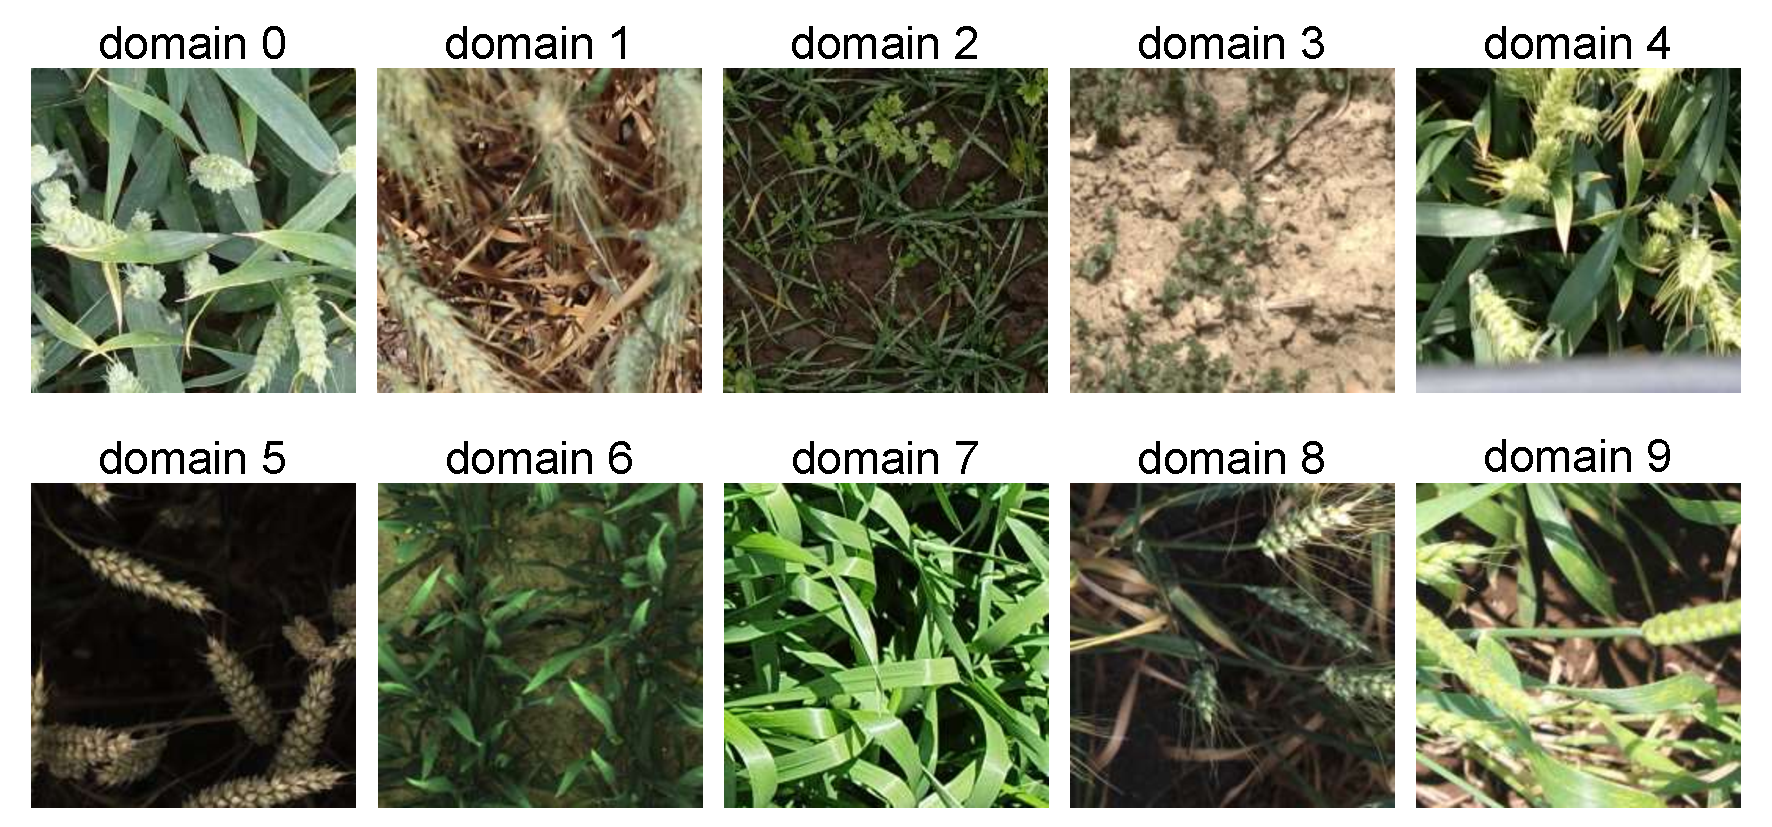
\includegraphics[width=\linewidth]{datasets.pdf}
    \caption{\textbf{Samples of different domains in the GWFSS dataset}. Domain 1-9 are used for training and validation, and domain 0 is used for testing. Different domains exhibit significant intrinsic and extrinsic variations.}
    \label{fig:dataset}
\end{figure}



